\documentclass[a4paper, titlepage, oneside]{article}
\usepackage[utf8]{inputenc}
\usepackage[australian]{babel}
\usepackage{csquotes}
\usepackage[vmargin = 2cm, hmargin = 2cm]{geometry}
\usepackage{amsmath,amssymb}
\usepackage{graphicx, epstopdf, listings, csvsimple, float, xcolor}
\usepackage[allcolors = blue, colorlinks = true, pdfpagemode = UseNone, pdfstartview = FitH]{hyperref}
\usepackage{multicol}
\usepackage{wasysym}
\usepackage[backend = biber, style = authoryear, alldates = iso8601]{biblatex}
\usepackage[cdot, amssymb]{SIunits}
\usepackage{aas_macros}

% listings, xcolor
\lstset{language=Matlab,
    commentstyle=\color{gray}\textit,
    stringstyle=\color{purple},
    showstringspaces=false,
    numbers=left,
    breaklines=true,
    breakatwhitespace=true,
    aboveskip=0pt,
    belowskip=20pt}

% Bibliography setup
\renewcommand{\nameyeardelim}{\addcomma\addspace} % Change delimiter for in-line citations to include a comma
\addbibresource{group-report.bib}

% inputenc : UTF-8 support for non-ASCII characters
% babel   : set language, for packages that need it
% csquotes  : context-sensitive quotes
% geometry  : page margins
% amsmath : maths
% amssymb : maths (\square redefined by siunits)
% graphicx  : \includegraphic
% epstopdf  : use of eps files in document
% hyperref  : in-document links
% listings  : import external code
% csvsimple : import csv tables
% float   : float graphics
% xcolor  : use colour formatting
% wasysym : \astrosun (conflict with amssymb)
% biblatex : bibliography
% SIunits : management of SI units; encourage using \unit{value}{units} command whenever possible

% Custom macros
\newcommand{\elem}[2]{\textsuperscript{#1}{#2}}
\newcommand{\molec}[2]{\ensuremath{\text{#1}_{#2}}}
\newcommand{\e}[1]{\ensuremath{\times 10^{#1}}}
\newcommand{\smass}{\mathrm{M_\odot}}
\newcommand{\parsec}{\mathrm{pc}}

% Document proper
\begin{document}
\title{\textbf{Searching for molecular gas towards TeV gamma-ray sources: Analysing 3D data cubes of the molecular gas tracer carbon monoxide with images from the HESS gamma-ray telescopes}}
\author{A.~K. Child \and R.~M. Harvey \and K.~T. Leaver \and H.~D. Poulter \and C.~M. Roe-Simons}
\date{7 October 2014} %Leave blank to print no date, or you can type in the desired date
\maketitle

\setcounter{page}{1}
\pagenumbering{roman}
\numberwithin{equation}{section}

\tableofcontents

\clearpage
\setcounter{page}{1}
\pagenumbering{arabic}

\begin{center}
  {\large \textbf{Searching for molecular gas towards TeV gamma-ray sources: Analysing 3D data cubes of the molecular gas tracer carbon monoxide with images from the HESS gamma-ray telescopes}}

  \vspace{1.5em}

  \textsc{A.~K. Child\footnote{Featured telescopes} \quad R.~M. Harvey\footnote{Molecular clouds and cosmic ray interactions} \quad K.~T. Leaver\footnote{\elem{12}{CO} and \elem{13}{CO} as tracers} \quad H.~D. Poulter\footnote{Galactic rotation} \quad C.~M. Roe-Simons\footnote{Cosmic ray sources}}
\end{center}

\vspace{1.5em}

\begin{minipage}{0.93\textwidth}
  \begin{abstract}
  This report is about finding the TeV sources and molecular clouds associated with such sources. It beings with a brief overview of the types of physical and astronomical concepts behind the science that has been used in writing up the report and making the conclusions. Bro!!
  \end{abstract}
\end{minipage}

\vspace{1em} % What the heck man this looks trash
% fuck u m8 every paper i've read has a neat space under the abstract


\begin{multicols}{2}
\section{Introduction}
\paragraph{}
Words words words, quick run-down of gamma rays and really high ones, just pretty much do a Gavin and copy stuff from Gavin's slides and so on and so forth.

\section{Theory}
\paragraph{}
Theory stuff goes in here, including but not limited to:
\begin{itemize}
  \item Cosmic ray sources
  \item Large molecular clouds, and their interactions with CRs
  \item CO \& \elem{13}{CO} as tracers
  \item Telescope information/general data stuff?
  \item Galactic rotation/Doppler shift in Mopra data
\end{itemize}
Fun! These titles are all outdated! We won't use these!

\subsection{Cosmic ray sources}
\paragraph{}
Go Coen! Goen! Wow that was awful!

\subsection{Molecular clouds}
\subsubsection{Composition and structure}
\paragraph{}
The average density of the interstellar medium (ISM) is quite low, however the reaches of space are littered with so-called molecular clouds -- areas with gas and dust density significantly higher, such that stars can form within the material. These clouds are predominantly composed of molecular hydrogen (\molec{H}{2}), which [as mentioned previously / for reasons to be discussed shortly] is relatively difficult to detect. However, the presence of carbon monoxide (CO) is significantly easier to determine, and astrophysicists presently believe it to be distributed among \molec{H}{2} in effectively equal quantities, making it an excellent tracer \parencite{Glover:2011}.

Gas and dust formations with a total mass between \(10^3\) and \unit{10^7}{\smass} are called giant molecular clouds (GMCs), and tend to be anywhere from 5 to 200 parsecs in diameter. \parencite{Murray:2011} ``Diameter'' is a term applied fairly loosely, as the form of a GMC is not guaranteed to be even remotely spherical. Indeed, the tenuous structural qualities of GMCs mean that they can also vary greatly in density, typically from around \(2\e{-20}\) to \unit{2\e{-18}}{\gram\usk\centi\metre\rpcubed}, corresponding to approximately \(10^4\) to \(10^6\) molecules per cubic centimetre \parencite{Ferriere:2001}.

\subsubsection{Interactions with cosmic rays}
\paragraph{}
Cosmic rays incident on GMCs can through a variety of mechanisms produce gamma rays, in our case often within TeV range and hence detectable by the HESS telescope. Bremsstrahlung radiation is motivated by Coulombic forces, and results from inbound cosmic rays being deflected by charged particles present in the interstellar gas, this change thus emitting gamma radiation. Inverse Compton scattering is motivated by conservation of momentum, and involves high-energy cosmic rays colliding with ``soft'' photons in the gas, exchanging momentum and in the process resulting in a more energetic photon with energies in TeV ranges \parencite{Ferriere:2001}. The synchrotron effect may also produce gamma rays, but is not included in this data set as HESS is not sensitive to such effects.

\subsubsection{Kinetic energy of expanding bubbles}
\label{sec:kinetic}
\paragraph{}
Powerful events in GMCs -- such as supernovae -- can push away all nearby gas, clearing out distinct ``bubble'' regions readily visible in images of gas distributions. In order to find the energy released by the event, we simply need find the kinetic energy of the gas which is now moving away, assuming it previously had negligible kinetic motion and almost all of the energy released by the event has been transferred to the surrounding gas.

The Mopra data cubes provide redshift speeds for each image slice, hence permitting us to find the relative speeds of two areas of gas, such as the two sides of an expanding bubble. For the full derivation please see Appendix~\ref{app:kinetic}, however the final result is replicated here:
\begin{equation}
  \mathrm{KE} = \frac{\pi ^ 4}{6} {\left( \frac{\Delta l}{360} \right)}^3 \rho d^3 {(v_1 - v_2)}^2 \, \joule \, ,
\end{equation}
where \(\Delta l\) is the maximum angular width of the bubble in degrees, \(\rho\) is an estimate of the mass density in \(\kilo\gram\usk\centi\metre\rpcubed\) of the gas previously occupying that volume, \(d\) is the distance to the centre of the bubble in \(\centi\metre\), and \(v_1\) and \(v_2\) are the redshift speeds of the front and back of the bubble in \(\metre\usk\reciprocal\second\).

\subsection{\elem{12}{CO} and \elem{13}{CO} as tracers}
\paragraph{}
\elem{12}{CO} henceforth CO blah blah. Kyle is going the extra mile in style! Friend, you have a good plan to make the works go forwards! More words just to make a larger paragraph!

\subsection{Featured telescopes}
\paragraph{}
Alisha ain't no child, no siree! I ran out of shitty announcer puns, forgive me! Tele-no-scope 360 xboxs swag!!!

More words! We need more words on this page! There's this problem I'm seeing where the paragraph spacing gets all wide and bad because \LaTeX~doesn't think there's enough here and stretches things out. Gotta have lotsa words.

\subsection{Galactic rotation}
\label{sec:gal-rot}
\paragraph{}
The Mopra data featured heavily in this report \parencite{Burton:2013} derives its usefulness from the effect that galactic rotation has on co-linear objects. Fig.~\ref{fig:gal-rot} shows how for a simplified model of the Milky Way with constant radial velocity, looking along a line of sight, in this particular instance one corresponding to a galactic latitude of \(l=337\), leads to a velocity gradient and a measurable Doppler shift. In order to find distances from the sun using the Mopra data, it is necessary to consider the component of velocity parallel to the line of sight. See Appendix~\ref{app:doppler} for the derivation. Hence, the velocity of an object along the line of sight with galactic latitude \(l\) is given by
\begin{equation}
  v_{los}(d)=\frac{v(R)R_0\sin{l}}{\sqrt{d^2-2R_0d\cos{l}+R_0^2}}-v(R_0)\sin{l}\;\,,
\end{equation}
where the distance from the sun to the galactic centre (GC) is \(R_0\), and distance from the sun to the object of interest is \(d\). This equation holds for a galaxy with variable rotation \(v(R)\) dependent on radial distance \(R\) from the GC, and for the sake of simplicity in this report is taken to be a constant \(v(R)=\unit{220}{\kilo\metre\usk\reciprocal\second}\) (CITE-REF). The distance from the GC is also taken to be \(R_0=\unit{8}{\kilo\parsec}\) (CITE-REF).

\begin{figure}[H]
  \centering
  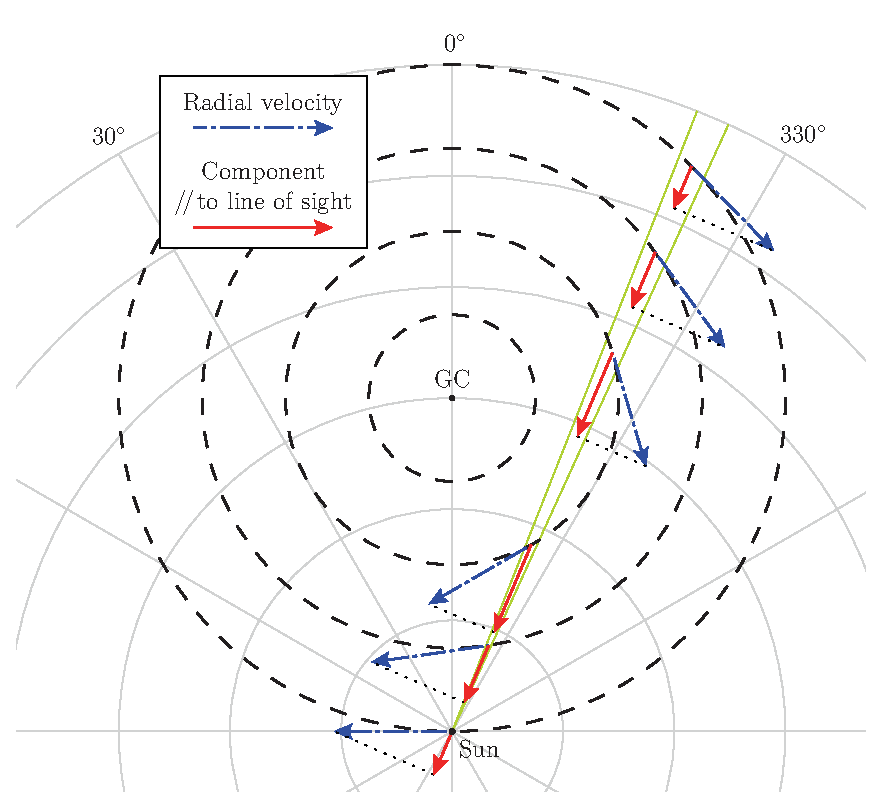
\includegraphics[width = 8cm]{figures/galactic-rotation}
  \caption{Galactic rotation showing Doppler shifts}
  \label{fig:gal-rot}
\end{figure}

\section{Data analysis}
\paragraph{}
Data analysis is coming first. We talk about many things including how we managed to reduce the noise in the \texttt{.fits} files we used to make the analysis. Yeas!

\subsection{Noise analysis}
\paragraph{}
Yes, keem em cumming!!

\section{Results and discussion}
\paragraph{}
This is where we talk aout all the resuts we get from our data analysis, probably a good idea to cover the data analysis first and all of that so that way things make more sense here. Results should relly not even be in here lel.

\subsection{Source candidates}
\paragraph{}
Here are some of the candidates for the gamma ray sources observed.

\subsubsection{HESS J1632-479}
\paragraph{}
Here are the things for this source. Probably include a picture of the source just as a nice ``here is thing''.

% I don't know if this is the best place for this stuff yet. It's kinda a result, kinda analysis
\subsection{IGR J16358-4726}
\paragraph{}
Also known as [KRL2007b] 194, this object is believed to be an x-ray binary, specifically of the variety which features a neutron star orbiting what is likely a main sequence star \parencite{Falanga:2011}. Etc etc this s-etc-ion under construction.

\section{Conclusions}
\paragraph{}
Bitch, we concluding now, making the statements that make a conclusion possible to be made with the words and the mouth. Bitch, we're flawless give us good grades.
\end{multicols}

\newpage

\appendix

\section{Derivation of kinetic energy of expanding bubble}
\label{app:kinetic}
\paragraph{}
Here we derive the equation found in Section~\ref{sec:kinetic}. We begin with the familiar nonrelativistic equation for kinetic energy,
\begin{equation}
  \mathrm{KE} = \frac{1}{2} m v ^ 2 \, ,
\end{equation}
where \(m\) is the mass of the material displaced by the bubble (typically somewhat of an estimate) and \(v\) is the speed at which the bubble is expanding, i.e., the average speed of the gas in the reference frame of the object presumed to be at the centre. Mass \(m\) is given by mass density \(\rho\) multiplied by volume \(V\), and \(v\) can be found by halving the difference in speeds \(v_1\) and \(v_2\) of the front and back of the bubble:
\begin{equation}
  \mathrm{KE} = \frac{1}{2} \rho V { \left( \frac{\lvert v_1 - v_2 \rvert}{2} \right) }^2 \, .
\end{equation}
The volume \(V\) of the bubble is given by its radius, hence,
\begin{equation}
  \mathrm{KE} = \frac{1}{8} \rho \left( \frac{4}{3}\pi r^3 \right) {(v_1 - v_2)}^2
\end{equation} \begin{equation}
  \mathrm{KE} = \frac{1}{6} \pi \rho r^3 {(v_1 - v_2)}^2  \, .
\end{equation}
To find the radius of the bubble, we first determine the image slice which is halfway between the front and back slices of the bubble, ideally giving us a view of the bubble's cross section at the centre. Using the formula outlined at the end of Appendix~\ref{app:doppler}, we can find the distance \(d\) to this slice. Now, consider a circle of radius \(d\) with its origin centred on the Solar System. This circle has a circumference of \(l = 2 \pi d\), and passes through all objects which are located a distance \(d\) away from us, including the middle of our chosen bubble. If we measure the angular width \(\Delta l\) of the bubble in degrees, then by a simple ratio the bubble has diameter \(\frac{\Delta l}{360}l\). Note this is diameter and not radius, so to get \(r\) we then halve this result. Thus,
\begin{equation}
  \mathrm{KE} = \frac{1}{6} \pi \rho {\left( \frac{1}{2} \frac{\Delta l}{360} 2 \pi d \right)}^3 {(v_1 - v_2)}^2  \, ,
\end{equation}
and we rearrange to get our final result:
\begin{equation}
  \mathrm{KE} = \frac{\pi ^ 4}{6} {\left( \frac{\Delta l}{360} \right)}^3 \rho d^3 {(v_1 - v_2)}^2 \, .
\end{equation}

\section{Derivation of galactic doppler shift}
\label{app:doppler}
\paragraph{}
Here we derive the equation found in Section~\ref{sec:gal-rot}. Looking at Fig.~\ref{fig:doppler}, we can (probably not) see the setup we're going to be dealing with here. In order to derive the velocity along the line of sight in the galactic plane, it is necessary to first consider the velocity field of the galactic plane. With coordinates centred on the GC, the velocity field can be expressed as
\begin{equation}
  \label{eq:vel-field}
  \mathbf{v}(x,y)=v(R)\cdot\!\left(\frac{y}{R},-\frac{x}{R}\right)\;,
\end{equation}
where \(x\), \(y\) are the Cartesian coordinates of point P, and \(R\) is the radial distance from point P to the GC, which by Pythagoras fulfils
\begin{equation}
  R^2=x^2+y^2\;.
\end{equation}

\begin{figure}
  \centering
  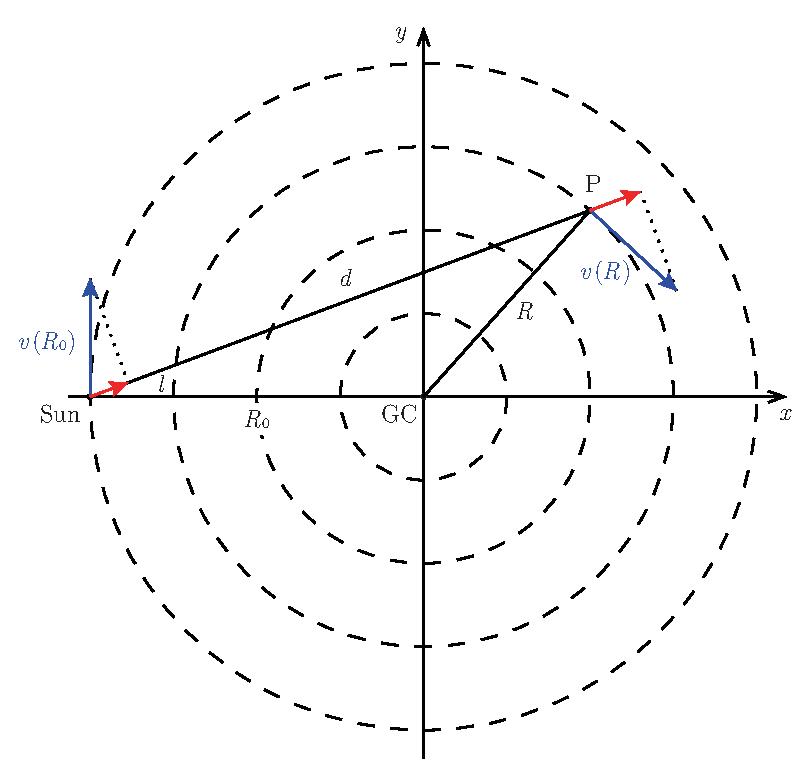
\includegraphics[width=13cm]{figures/doppler-shift}
  \caption{Velocity along line of sight in the galactic plane}
  \label{fig:doppler}
\end{figure}

In Eq.~\eqref{eq:vel-field}, \(v(R)\) is the radial velocity at point P with dependence on \(R\). This velocity field has galactic radial velocities pointing counter clockwise, which is what would be expected of a model for the Milky Way. In order to compute the component of velocities along the line of sight, it is worth considering first the dot product of the velocity field with the direction vector in the direction of the line of sight, \(\mathbf{\hat{d}}\):
\begin{align}
  \mathbf{v}(x,y)\cdot\mathbf{\hat{d}}&=v(R)\left[\left(\frac{y}{R},-\frac{x}{R}\right)\!\cdot(\cos{l},\sin{l})\right] \\
  &=v(R)\left(\frac{y\cos{l}-x\sin{l}}{R}\right) \\
  &=v(R)\left(\frac{y\cos{l}-x\sin{l}}{\sqrt{x^2+y^2}}\right)\;.
  \label{eq:vel-dot}
\end{align}
This expression gives the component of velocity in the \(\mathbf{\hat{d}}\) direction for any \((x,y)\). In order for this expression to be of any use in calculating the Doppler shift from the Mopra data, the coordinates need to be constained to the line of sight. The equation for the line of sight is given in vector form as:
\begin{equation}
  \lambda(d,l)=(d\cos{l}-R_0,d\sin{l})\;\,.
\end{equation}
Substituting the \(x\)- and \(y\)-coordinates from this expression in to Eq.~\eqref{eq:vel-dot} and expanding gives
\begin{equation}
  v_{los}(d)=\frac{v(R)R_0\sin{l}}{\sqrt{d^2-2R_0d\cos{l}+R_0^2}}\;\,.
\end{equation}
This expression only yields the absolute motion in the galaxy, and it is easy to see that for \(d=0\), \(v(0)=v(R)\sin{l}\) -- the sun's component of velocity along the line of sight. Subtracting this value gives us the equation used in the analysis of Mopra data:
\begin{equation}
  v_{los}(d)=\frac{v(R)R_0\sin{l}}{\sqrt{d^2-2R_0d\cos{l}+R_0^2}}-v(R_0)\sin{l}\;\,.
\end{equation}

\printbibliography[heading = bibintoc] % Include bibliography entry in ToC

\end{document}